\documentclass{report}
\usepackage[margin=1in, paperwidth=8.5in, paperheight=11in]{geometry}
%Math packages%
\usepackage{amsmath}
\usepackage{amsthm}
%Spacing%
\usepackage{setspace}
\onehalfspacing
%Lecture number%
\newcommand{\lectureNum}{6}
%Variables - Date and Course%
\newcommand{\curDate}{January 16, 2017}
\newcommand{\course}{MATH 239}
\newcommand{\instructor}{Luke Postle}
%Defining the example tag%
%\theoremstyle{definition}%
\newtheorem{ex}{Example}[section]
%Setting counter given the lecture number%
\setcounter{chapter}{\lectureNum{}}
%Package for drawing graphs%
\usepackage{tikz}
\usepackage{verbatim}
\usetikzlibrary{arrows}

\begin{document}
%Note title%
\begin{center}
\begin{Large}
\textsc{\course{} | Lecture \lectureNum{}}
\end{Large}
\end{center} 
\noindent \textit{Bartosz Antczak} \hfill
\textit{Instructor: \instructor{}} \hfill
\textit{\curDate{}}
\rule{\textwidth}{0.4pt}

% Actual Notes%
\subsubsection{Review of last lecture}
\textbf{Path-connectedness} (whether two vertices are connected by a path) is an equivalence relation. The equivalence classes are called the \underline{components} of $G$. A graph is connected if and only if it has one component.
\section{Algorithmic Questions for Connectedness}
%polynomiL VS. exponential (i.e., brute force is more exponential)%
When we study algorithmic questions, we often ask ourselves about how efficient they are. Another topic to focus on is how efficiently can we \textit{confirm} that the algorithm is correct, from this stems the idea of $P$ and $NP$ (and also co-$NP$):
\begin{itemize}
\item $P$ (polynomial time) | an algorithm that runs in time polynomial of its input
\item $NP$ (non-deterministic polynomial time) | checking whether an algorithm is correct (i.e., if the output of a certain algorithm is correct, I can convince you in polynomial time that it's correct, or equivalently if I'm allowed to guess as much as I want for free, it's in $P$)
\item Co-$NP$ | checking whether the output of an algorithm is incorrect (i.e., I can convince you that the answer is incorrect, thus there being no solution, in polynomial time)
\end{itemize}
Since most students in this class are CS majors, we'll focus on this approach to analysing problems in graph theory.
\subsubsection{Definition | ``Cut"}
\noindent Let $X \subseteq V(G)$. The \textit{cut} induced by $X$ is the set of edges with one end in $X$ and the other not in $X$. This set is denoted $\delta(X)$. 
\begin{ex}
Consider the following graph. If we let $X = \{1, 2, 3\}$, then $\delta(X) = \{25, 34\}$, which are the two edges that link the rest of the graph with $X$.
\end{ex}
%Graph 1%
\begin{center}
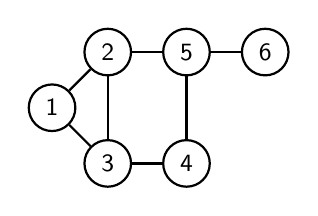
\begin{tikzpicture}[-,auto,node distance=1cm,
                    thick,main node/.style={circle,draw,font=\sffamily\small}]
  %C_4%
  \node[main node] (1) {1};
  \node[main node] (2) [above right of=1] {2};
  \node[main node] (3) [below right of=1] {3};
  \node[main node] (4) [right of=3] {4};
  \node[main node] (5)[right of=2] {5};
  \node[main node] (6)[right of=5] {6};
    
  \path[every node/.style={font=\sffamily\small}]
    (1) edge node [left] {} (2)
    	edge node [below] {} (3)
    (2) edge (5)
    	edge (3)
    (3) edge (4)
    (4) edge (5)
    (5) edge (6);
\end{tikzpicture}
\end{center}
\subsubsection{Theorem 1}
\begin{center}
\textit{$G$ is disconnected if and only if there exists a proper, non-empty set $X$ of $V(G)$ such that the cut induced by $X$ is empty.}
\end{center}
\underline{\textbf{Proof:}} To prove this, we must show that this statement holds in both ``directions" (since it's an iff statement). The proof will conclude on the next page. \newpage
\textit{(proof of theorem 1 continued)}
\begin{itemize}
\item Proof in the $\implies$ direction: \textit{if $G$ is disconnected, there there exists such a cut.}\\
Since $G$ is disconnected, $G$ has at least two components. Let $X$ be te set of vertices of one component of $G$. Then $\delta(X)$ is empty since there are no edges between different components.
\item Proof in the $\impliedby$ direction: \textit{if there exists a cut, then $G$ is disconnected}.\\Suppose not (we're going by contradiction). Let $u$ be a vertex in $X$ and $v$ not in $X$ ($u$ exists since $X$ is non-empty, and $v$ exists since $X$ is proper). Since we suppose $G$ \textit{is} connected, there exists a path $P$ from $u$ to $v$, but then there exists an edge $e \in P$ with one end in $X$ and the other not in $X$, contradicting that $\delta(X)$ is empty.
\end{itemize}
\subsubsection{Proving Whether a Graph is Connected or Not}
To prove a graph $G$ is
\begin{itemize}
\item \textit{disconnected}: use the previous theorem and exhibit such a set $X$ that satisfies the requirements for a disconnected graph
\item \textit{connected}: show that there exists a path between every pair of vertices (but \underline{actually} only need a path from one vertex to rest of the vertices, or in other words a ``common central point" in the graph; refer to theorem 2) 
\end{itemize}
\subsubsection{Theorem 2}
\begin{center}
\textit{If $v \in V(G)$ and there is a path from  $v$ to every vertex of $G$, then $G$ is connected.}
\end{center}
\underline{\textbf{Proof:}} Let $u, w \in V(G)$. By our assumption, there exists a path from $v$ to $u$ and also from $v$ to $w$. We can connect the two paths to form a link from $w$ to $v$, and then from $v$ to $u$. If this link is a path, we have proven that there exists a path between any two pairs of vectors in $G$, thus showing that $G$ is connected. If the link is a walk, using a corollary proven in lecture 4, any walk can be converted to a path, and thus we arrive at the same conclusion.
\section{Trees and Forests}
\subsection{Definition:} A graph is a \textbf{forest} if it contains no cycles. A graph is a \textbf{tree} if it's a \textit{connected} forest. Every tree is a forest (converse not true), and every component of a forest is a tree.\subsubsection{Proposition}
\begin{center}
\textit{If $H$ is a subgraph of a forest $G$, then $H$ is a forest.}
\end{center}
\underline{\textbf{Proof:}}
Suppose not. Then $H$ contains a cycle, call it $C$. But if $G$ contains $C$, then $G$ is not a forest | a contradiction.\\\\
Final note: it's not true that every subgraph of every tree is itself a tree.
%END%

\end{document}